\section{Família de Curvas sob Controle Escalar com Relação $V/f$ Constante}\label{sec:controle_escalar}

O acionamento de máquinas de indução com velocidade ajustável mediante inversores de frequência fundamenta-se na manutenção da densidade de fluxo magnético no entreferro através da modulação proporcional entre a amplitude de tensão e a frequência fundamental da alimentação. A análise da família de curvas de conjugado resultante permite verificar a preservação da capacidade de sobrecarga e quantificar os efeitos degradantes da queda resistiva estatórica em baixas rotações.

% =========================================================================
% [DIRETRIZ DE REDAÇÃO]
% - Objetivo: Atender ao Item 1.F de sim_proj.pdf. Emular a operação com inversor de
%   frequência sob controle escalar (V/f constante) nos patamares de 100%, 75%, 50% e 25%.
% - Formulação: Demonstrar a proporcionalidade do fluxo de entreferro \Phi_{ag} \propto V/f = constante.
%   Explicar a velocidade síncrona proporcional à frequência (n_s = 1800, 1350, 900 e 450 rpm)
%   e o efeito da queda resistiva no estator (queda IR_1) em baixas frequências (15 Hz).
% - Figuras/Tabelas: Inserir a figura comparativa com as 4 curvas sobrepostas: item1f_vf_scalar_family.png.
% - Confronto: Analisar a degradação progressiva do conjugado máximo (T_max de 54,63 N*m a 30,65 N*m),
%   justificando a necessidade de compensação de tensão (voltage boost) em acionamentos industriais.
% =========================================================================

\subsection{Princípio do Controle Escalar e Manutenção do Fluxo de Entreferro}\label{subsec:principio_vf}

A força eletromotriz induzida no estator pelo campo magnético girante relaciona-se com o fluxo de pico por polo ($\Phi_{ag}$) pela Lei de Faraday-Neumann:
\begin{equation}
E_1 = \sqrt{2} \pi f_1 N_1 k_{w1} \Phi_{ag} \approx V_1,
\label{eq:fem_faraday_fluxo}
\end{equation}
em que $N_1$ representa o número de espiras em série por fase e $k_{w1}$ o fator de enrolamento fundamental. Desprezando-se em primeira aproximação a queda de tensão na impedância primária, o fluxo magnético no entreferro é diretamente proporcional à razão entre a tensão e a frequência fundamental da rede:
\begin{equation}
\Phi_{ag} \propto \frac{V_1}{f_1} = \frac{\SI{220}{\volt}}{\SI{60}{\hertz}} \approx \SI{3,6667}{\volt/\hertz}.
\label{eq:razao_vf}
\end{equation}

A manutenção dessa relação constante assegura que o núcleo ferromagnético opere próximo ao seu joelho de saturação de projeto, viabilizando o desenvolvimento do mesmo conjugado máximo independente da rotação operacional. A velocidade síncrona do campo girante ($n_s$) desloca-se linearmente com a frequência imposta pelo inversor:
\begin{equation}
n_s(f) = \frac{120 \cdot f}{p}.
\label{eq:ns_frequencia}
\end{equation}

Para a avaliação comparativa prescrita no projeto acadêmico, definem-se quatro patamares proporcionais de frequência e tensão de alimentação:
\begin{enumerate}
    \item \textbf{100\% (Nominal):} $f = \SI{60}{\hertz}$, $V_L = \SI{220}{\volt}$, $n_s = \SI{1800}{\RPM}$;
    \item \textbf{75\%:} $f = \SI{45}{\hertz}$, $V_L = \SI{165}{\volt}$, $n_s = \SI{1350}{\RPM}$;
    \item \textbf{50\%:} $f = \SI{30}{\hertz}$, $V_L = \SI{110}{\volt}$, $n_s = \SI{900}{\RPM}$;
    \item \textbf{25\%:} $f = \SI{15}{\hertz}$, $V_L = \SI{55}{\volt}$, $n_s = \SI{450}{\RPM}$.
\end{enumerate}

\subsection{Inspeção da Família de Curvas e Efeito da Resistência Estatórica}\label{subsec:analise_familia_vf}

A \Cref{fig:familia_vf} apresenta a família de curvas características de conjugado eletromagnético em função da velocidade mecânica calculadas para os quatro patamares operacionais.

\begin{figure}[H]
\centering
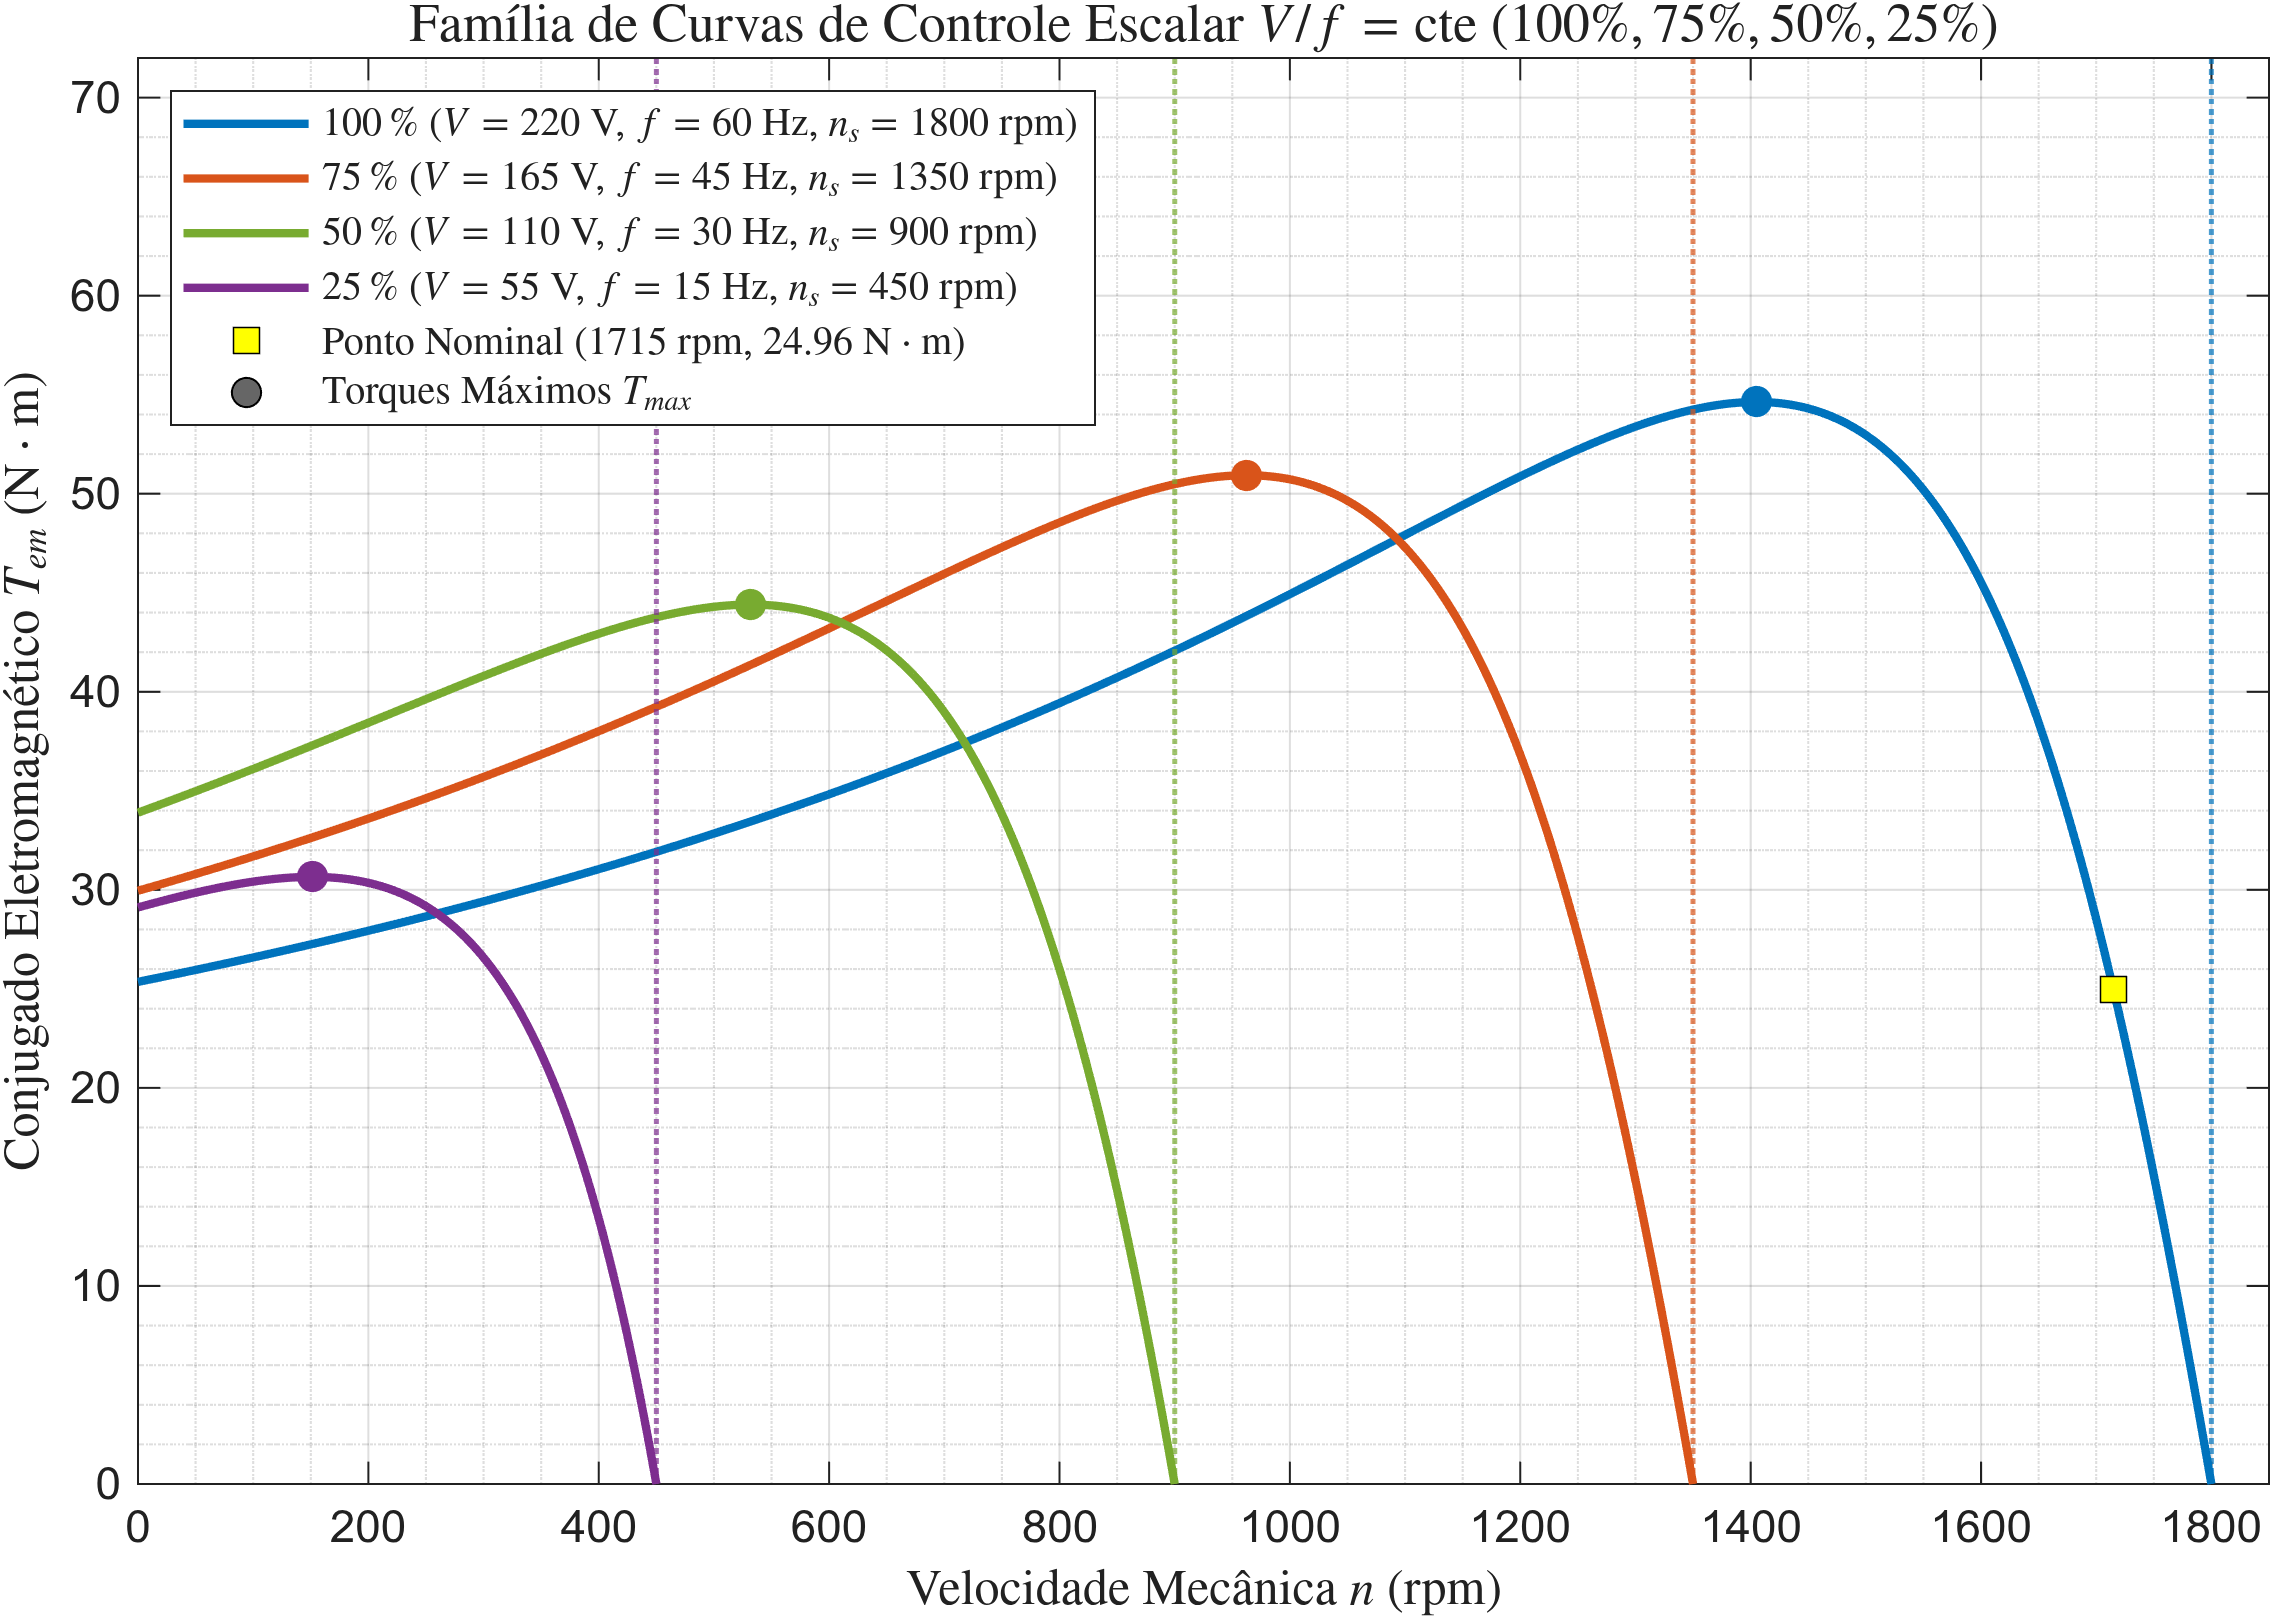
\includegraphics[width=0.88\textwidth]{item1f_vf_scalar_family.png}
\caption{Família de curvas características de Conjugado versus Velocidade sob controle escalar $V/f$ constante ($100\%$, $75\%$, $50\%$ e $25\%$).}
\label{fig:familia_vf}
\end{figure}

A \Cref{tab:pontos_notaveis_vf} consolida os marcadores numéricos extraídos analiticamente para cada patamar de modulação $V/f$.

\begin{table}[H]
\centering
\caption{Marcadores numéricos de desempenho da família de curvas sob controle escalar $V/f$.}
\label{tab:pontos_notaveis_vf}
\resizebox{\textwidth}{!}{%
\begin{tabular}{cccccc}
\toprule
\textbf{Patamar} & \textbf{Frequência ($f$)} & \textbf{Tensão ($V_L$)} & \textbf{Síncrona ($n_s$)} & \textbf{Conjugado Máx. ($T_{max}$)} & \textbf{Rotação em $T_{max}$} \\
\midrule
\SI{100}{\percent} & \SI{60}{\hertz} & \SI{220}{\volt} & \SI{1800}{\RPM} & \SI{54,633}{\Nm} & \SI{1405,2}{\RPM} \\
\SI{75}{\percent}  & \SI{45}{\hertz} & \SI{165}{\volt} & \SI{1350}{\RPM} & \SI{50,933}{\Nm} & \SI{962,7}{\RPM} \\
\SI{50}{\percent}  & \SI{30}{\hertz} & \SI{110}{\volt} & \SI{900}{\RPM}  & \SI{44,402}{\Nm} & \SI{531,9}{\RPM} \\
\SI{25}{\percent}  & \SI{15}{\hertz} & \SI{55}{\volt}  & \SI{450}{\RPM}  & \SI{30,652}{\Nm} & \SI{151,3}{\RPM} \\
\bottomrule
\end{tabular}%
}
\end{table}

A inspeção dos dados revela que, em uma máquina puramente ideal ($R_1 = 0$), o conjugado máximo seria rigorosamente invariante com a frequência:
\begin{equation}
T_{max,\text{ideal}} \approx \frac{3 V_{th}^2}{2\omega_s (X_{th} + X_2')} \propto \frac{(V/f)^2}{(X/f)} = \text{constante}.
\label{eq:tmax_ideal_invariante}
\end{equation}

Contudo, na máquina física real de \SI{3,7}{\kilo\watt}, a resistência estatórica possui valor constante ($R_1 = \SI{1,189}{\ohm}$), independente da frequência de excitação. À medida que a frequência se reduz, as reatâncias indutivas de dispersão e magnetização decrescem proporcionalmente ($X = 2\pi f L$), enquanto a resistência $R_1$ permanece fixa. Consequentemente, a queda ôhmica de tensão no estator ($I_1 R_1$) passa a consumir uma fração cada vez mais expressiva da tensão aplicada:
\begin{itemize}
    \item A \SI{60}{\hertz} ($V_L = \SI{220}{\volt}$), a queda $I_1 R_1$ representa pequena fração da tensão de fase e $T_{max} = \SI{54,633}{\Nm}$.
    \item A \SI{15}{\hertz} ($V_L = \SI{55}{\volt}$), a queda resistiva no enrolamento estatórico consome parcela substancial da tensão terminal, deprimindo a amplitude da força eletromotriz de entreferro ($E_1$) e enfraquecendo a densidade de fluxo $\Phi_{ag}$.
\end{itemize}

Esse enfraquecimento de campo em baixas velocidades acarreta uma degradação severa no conjugado máximo de desengate, que decai de \SI{54,633}{\Nm} (a \SI{60}{\hertz}) para \SI{30,652}{\Nm} (a \SI{15}{\hertz}), uma redução de \SI{43,9}{\percent} na capacidade de sobrecarga mecânica.

\subsection{Compensação de Tensão em Baixas Rotações (\textit{Voltage Boost})}\label{subsec:voltage_boost}

Para superar a degradação do conjugado induzida pela resistência primária em inversores industriais modernos, implementa-se a técnica de reforço de tensão de partida (\textit{voltage boost}). A curva de modulação escalar é corrigida por uma componente de offset em baixa frequência:
\begin{equation}
V_1(f) = V_{\text{boost}} + k_v \cdot f,
\label{eq:voltage_boost_formula}
\end{equation}
na qual o patamar $V_{\text{boost}}$ compensa exatamente a queda de tensão resistiva $I_1 R_1$ a velocidade nula, restabelecendo a densidade nominal de fluxo de entreferro ($\Phi_{ag} \approx \text{cte}$) e restaurando o conjugado máximo pleno de \SI{54,6}{\Nm} desde as frequências mais baixas de partida. Em acionamentos de alto desempenho dinâmico, essa limitação do controle escalar constitui a principal justificativa técnica para a transição para esquemas de Controle Vetorial por Orientação de Campo (FOC).
